

\chapter{Chapitre}
	\section{Section} \label{ref_section}
		\subsection{Sous Section}
			\subsubsection{Sous Section}

\chapter{Graphiques}

	\begin{tikzpicture}
		\begin{axis}[
				title={TITLE},
				xlabel={legende X},
				% xmode=lin,
				ylabel={legende Y},
				% ymax=110,
				mark size=0.5pt,
				width=1\textwidth,
				legend style={at={(0.5,-0.15)},anchor=north},
				legend columns=5,
			]
			\addplot [red,thick] table {tex/std/data_base.txt};
			\legend{output},
		\end{axis}
	\end{tikzpicture}

% data_base.txt
% x1 y1
% x2 y2
% x3 y3


\chapter{Text Barrés}
	text normal, \sout{texte à barrer}, \xout{texte à hachurer} et text normal

%
% hyperref : pdf editables : https://la-bibliotex.fr/2020/04/11/creer-des-pdf-editables-avec-latex/
%

\chapter{Formulaires}
	\section{Champs}
		\formfield[10cm]{Mme/M. :}
		\formfield[10cm]{Adresse :}
		\formfield[10cm]{Code postal :}


	\section{Checbox}
		\begin{itemize}
			\item \tikzcheckmark{}
			\item \tikzcheckmark{no mark}
			\item \tikzcheckmark{mark}
			\item \tikzcheckmark{bad mark}
		\end{itemize}

	\section{Note}
		Les formulaires interactifs ne sont pas possible sans utiliser PDFlatex, ici, ce n'est pas considéré
% 	\begin{Form}
% 		\TextField{Mme/M. : }
% 		\CheckBox{Case à cocher : }
% 		\ChoiceMenu[combo]{Âge :}{
% 			0--18 ans,
% 			18--45,
% 			45--65,
% 			plus de 65
% 			}
% 	\end{Form}

\chapter{Multi figures}
	\begin{figure}[H]
		\center
		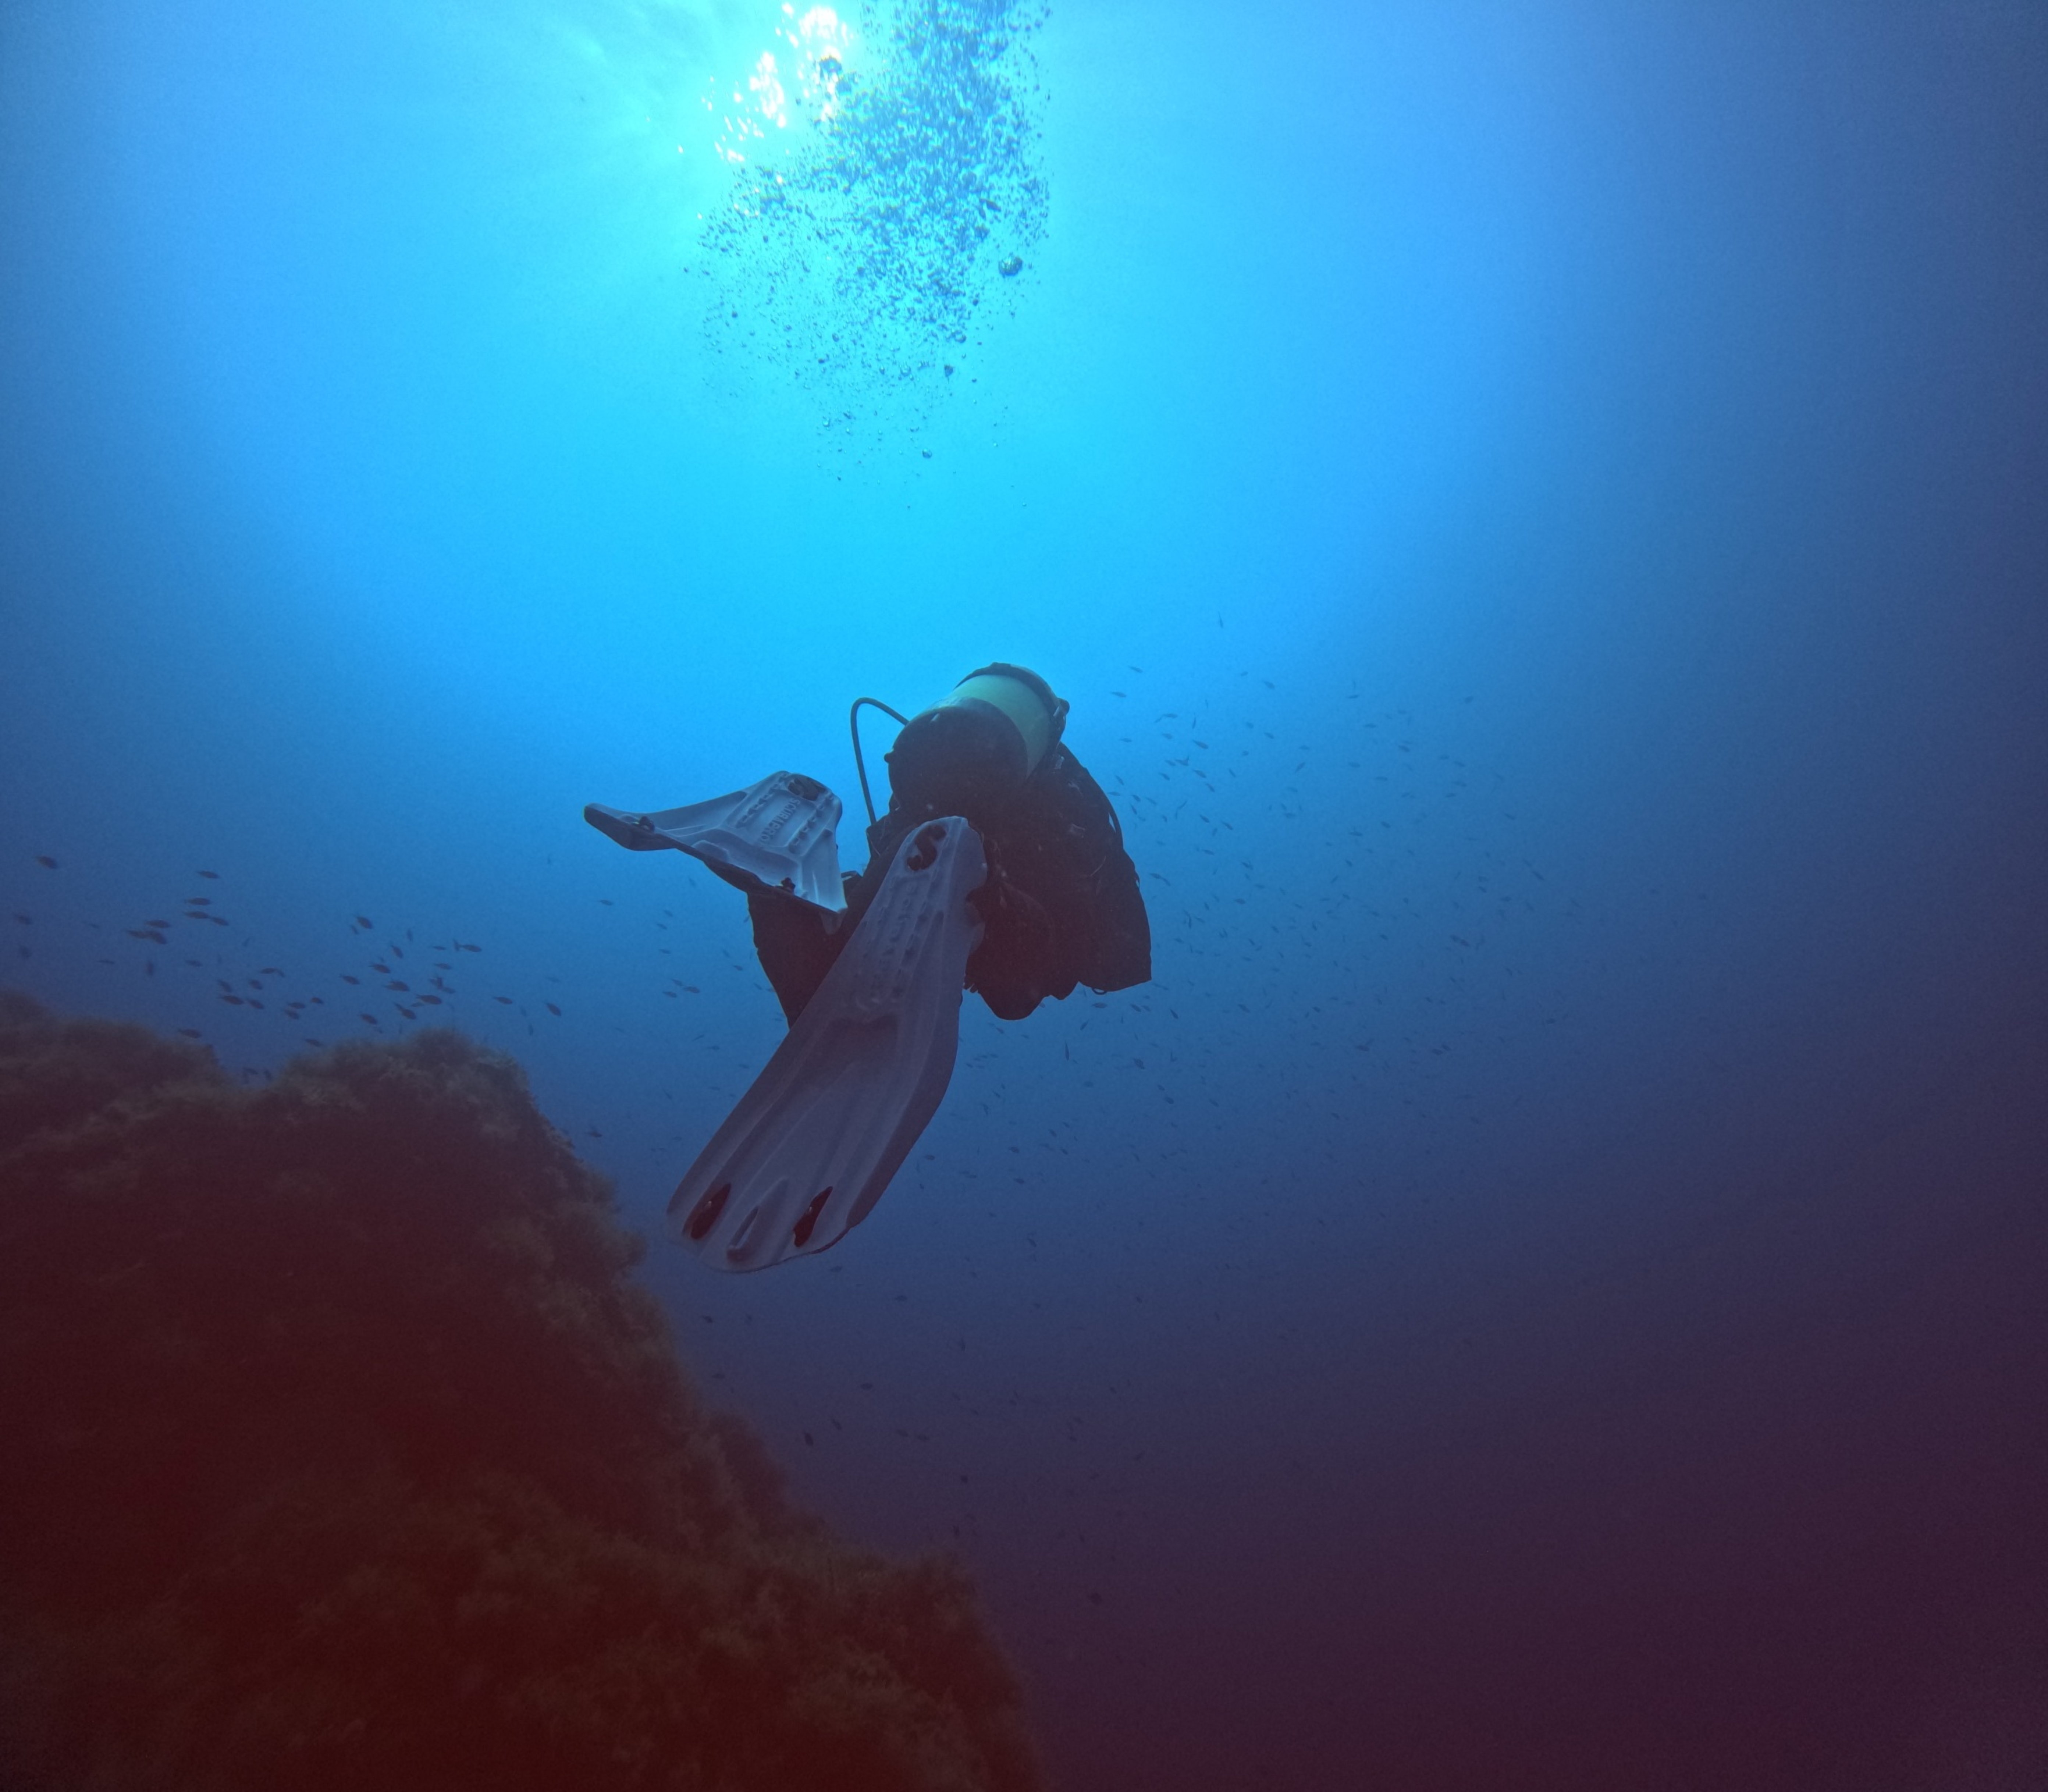
\includegraphics[width=50mm]{res/img}
		\caption{Légende pour une figure}
	\end{figure}

	\begin{figure}
		\centering % pour centrer l’ensemble
		\subfloat[sous-légende 1]{
			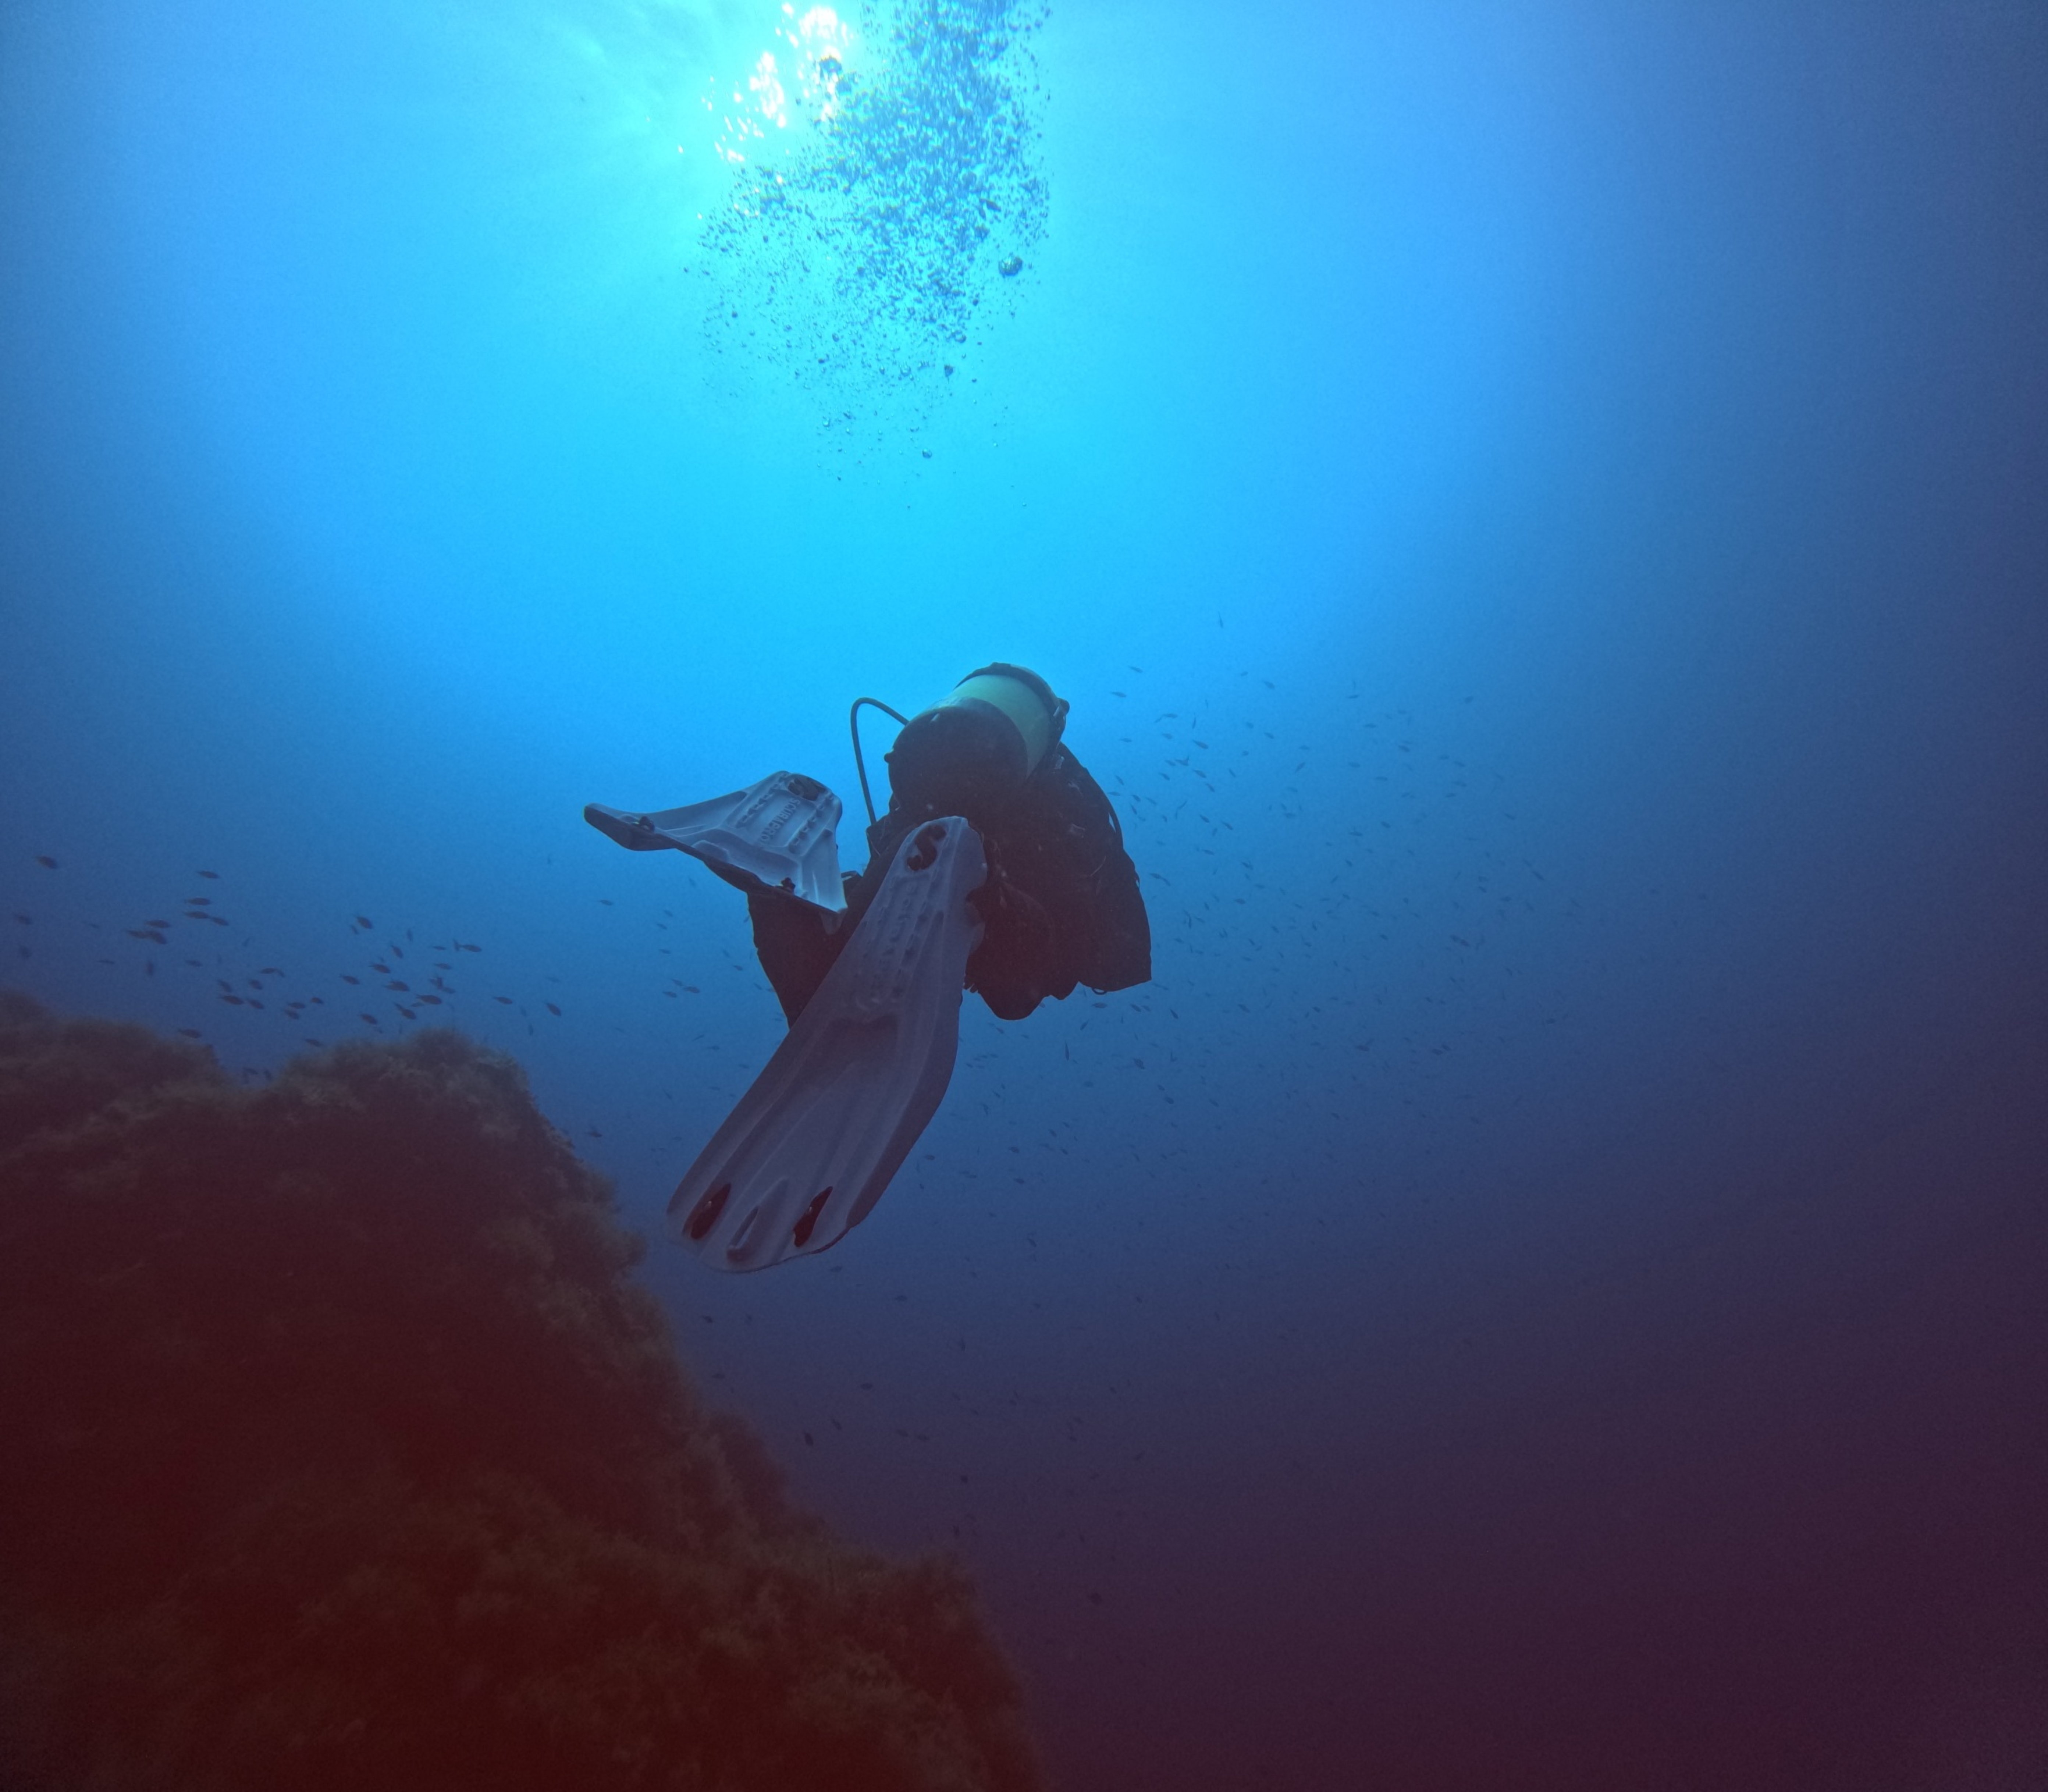
\includegraphics[scale=0.01]{res/img}
			\label{label_sous_figure_1}
		}
		\subfloat[sous-légende 2]{
			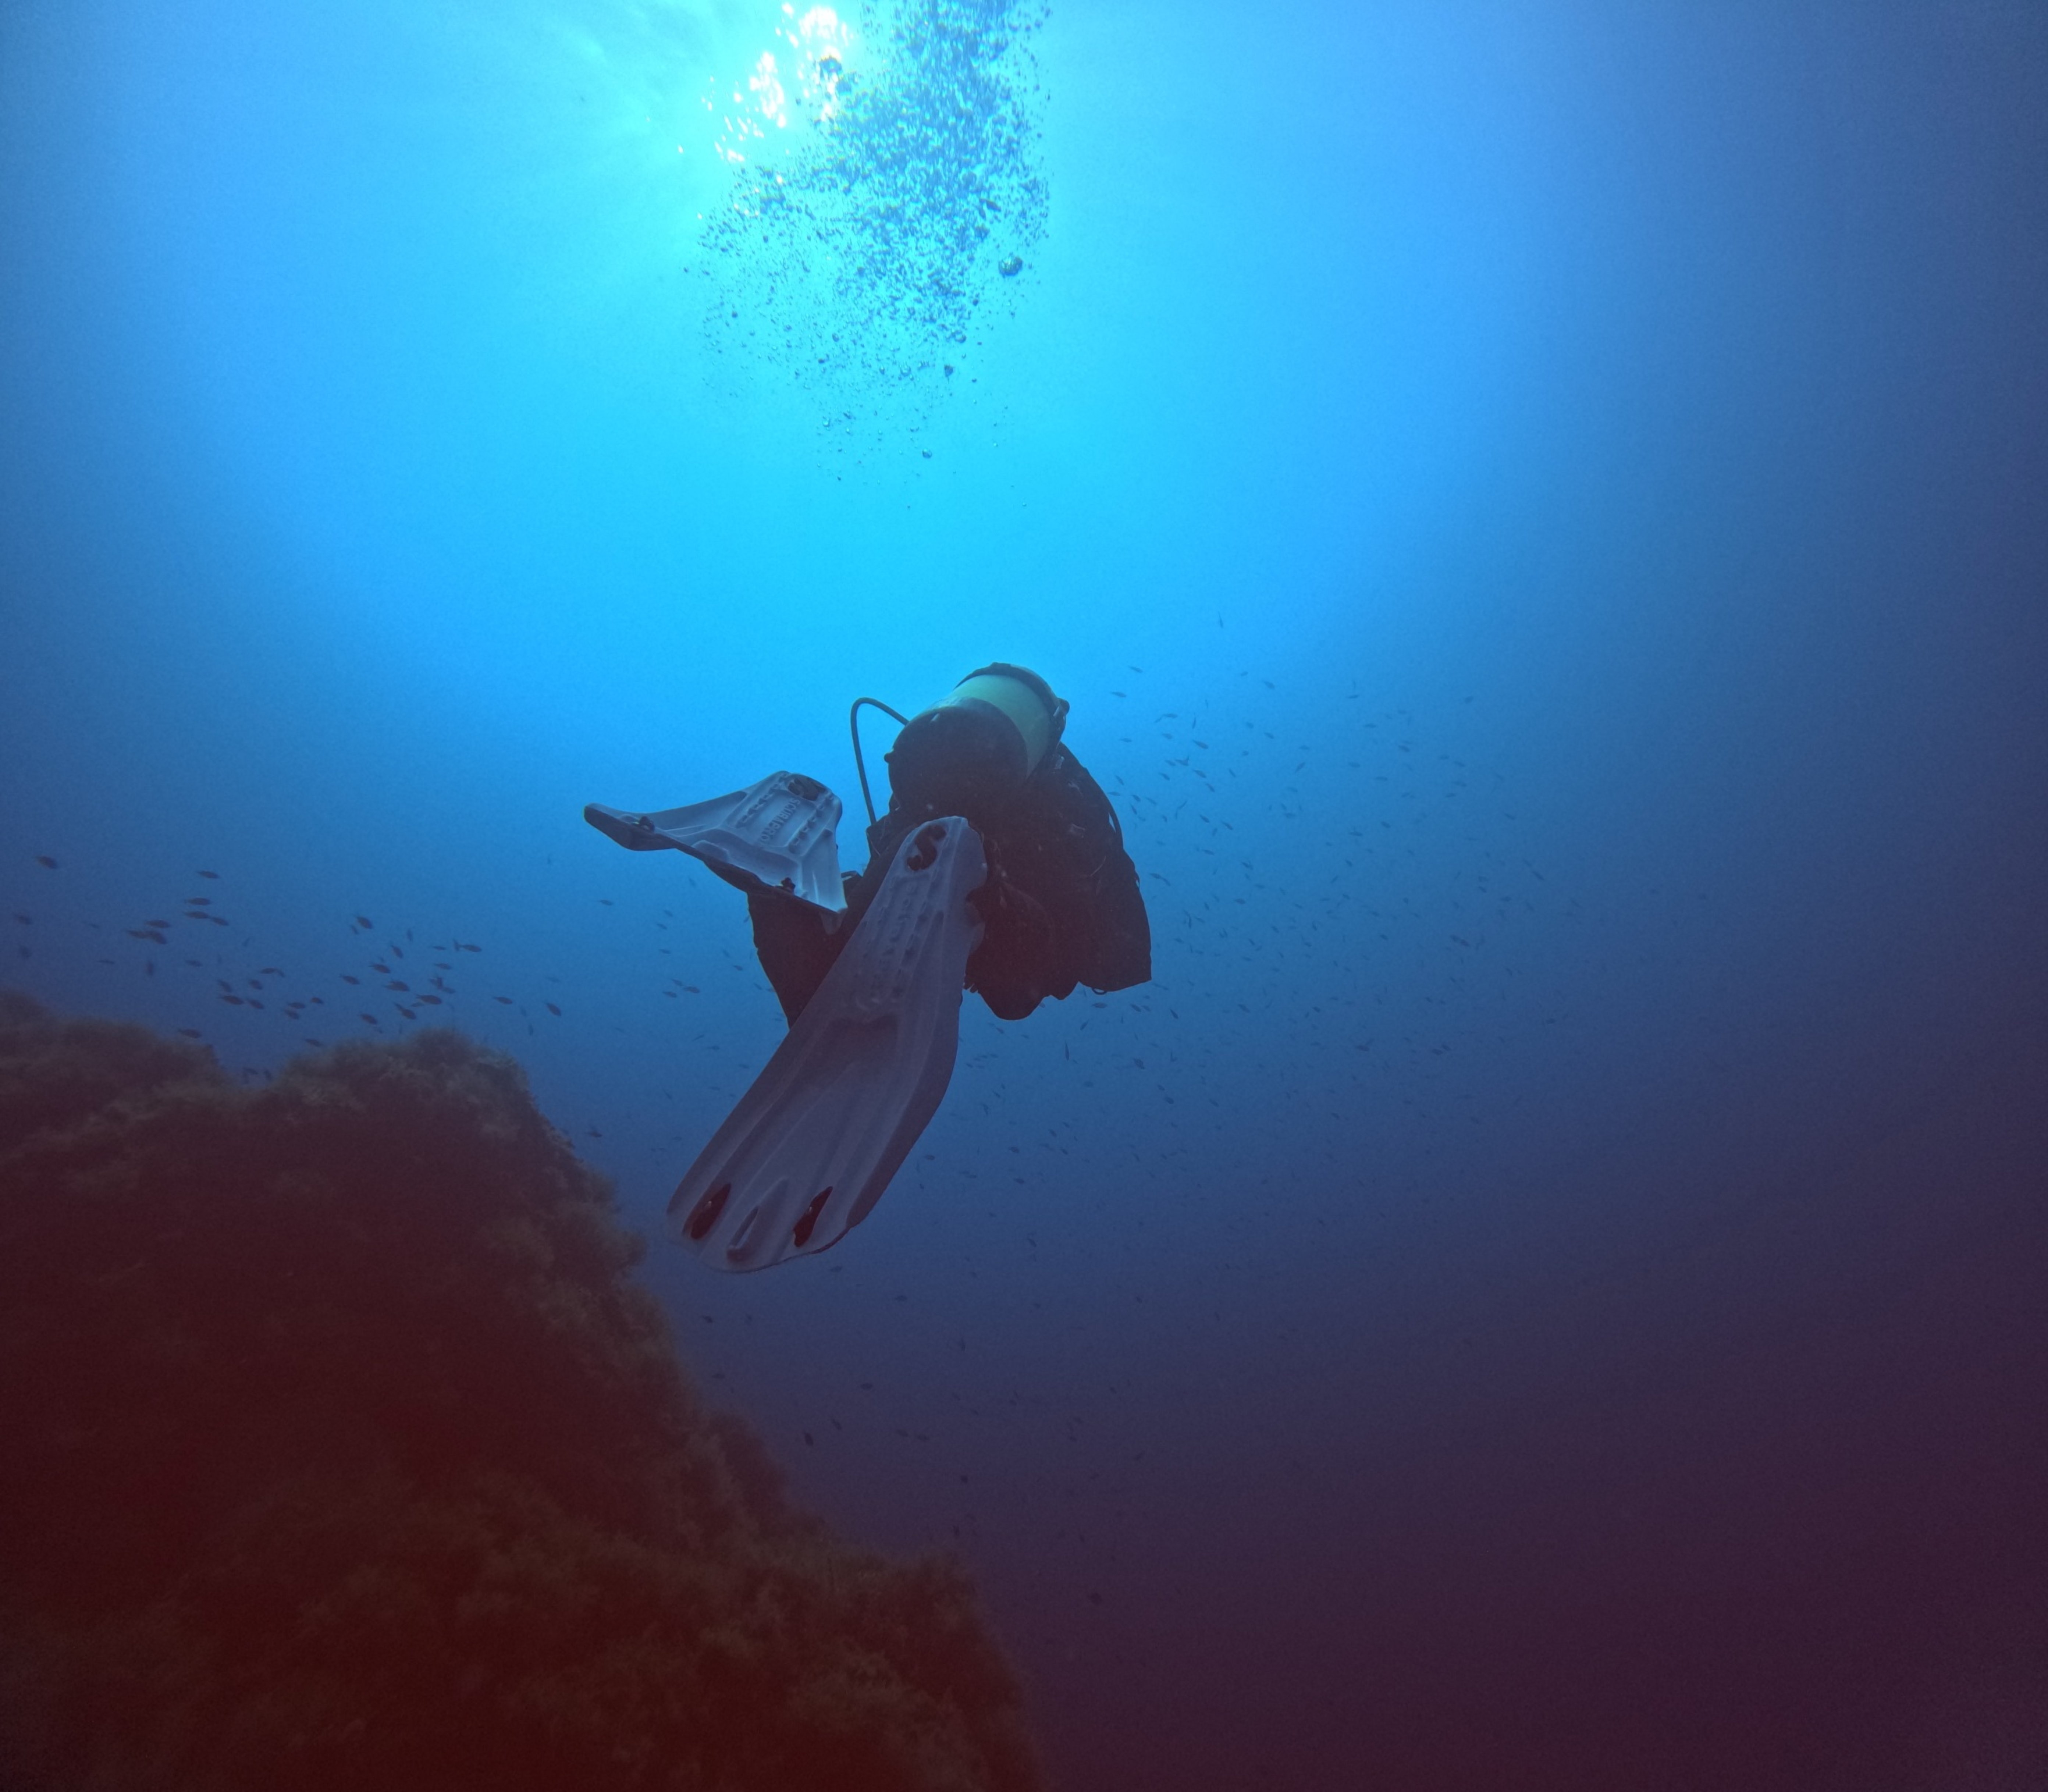
\includegraphics[scale=0.01]{res/img}
			\label{label_sous_figure_2}
		}\\
		\subfloat[sous-légende 3]{
			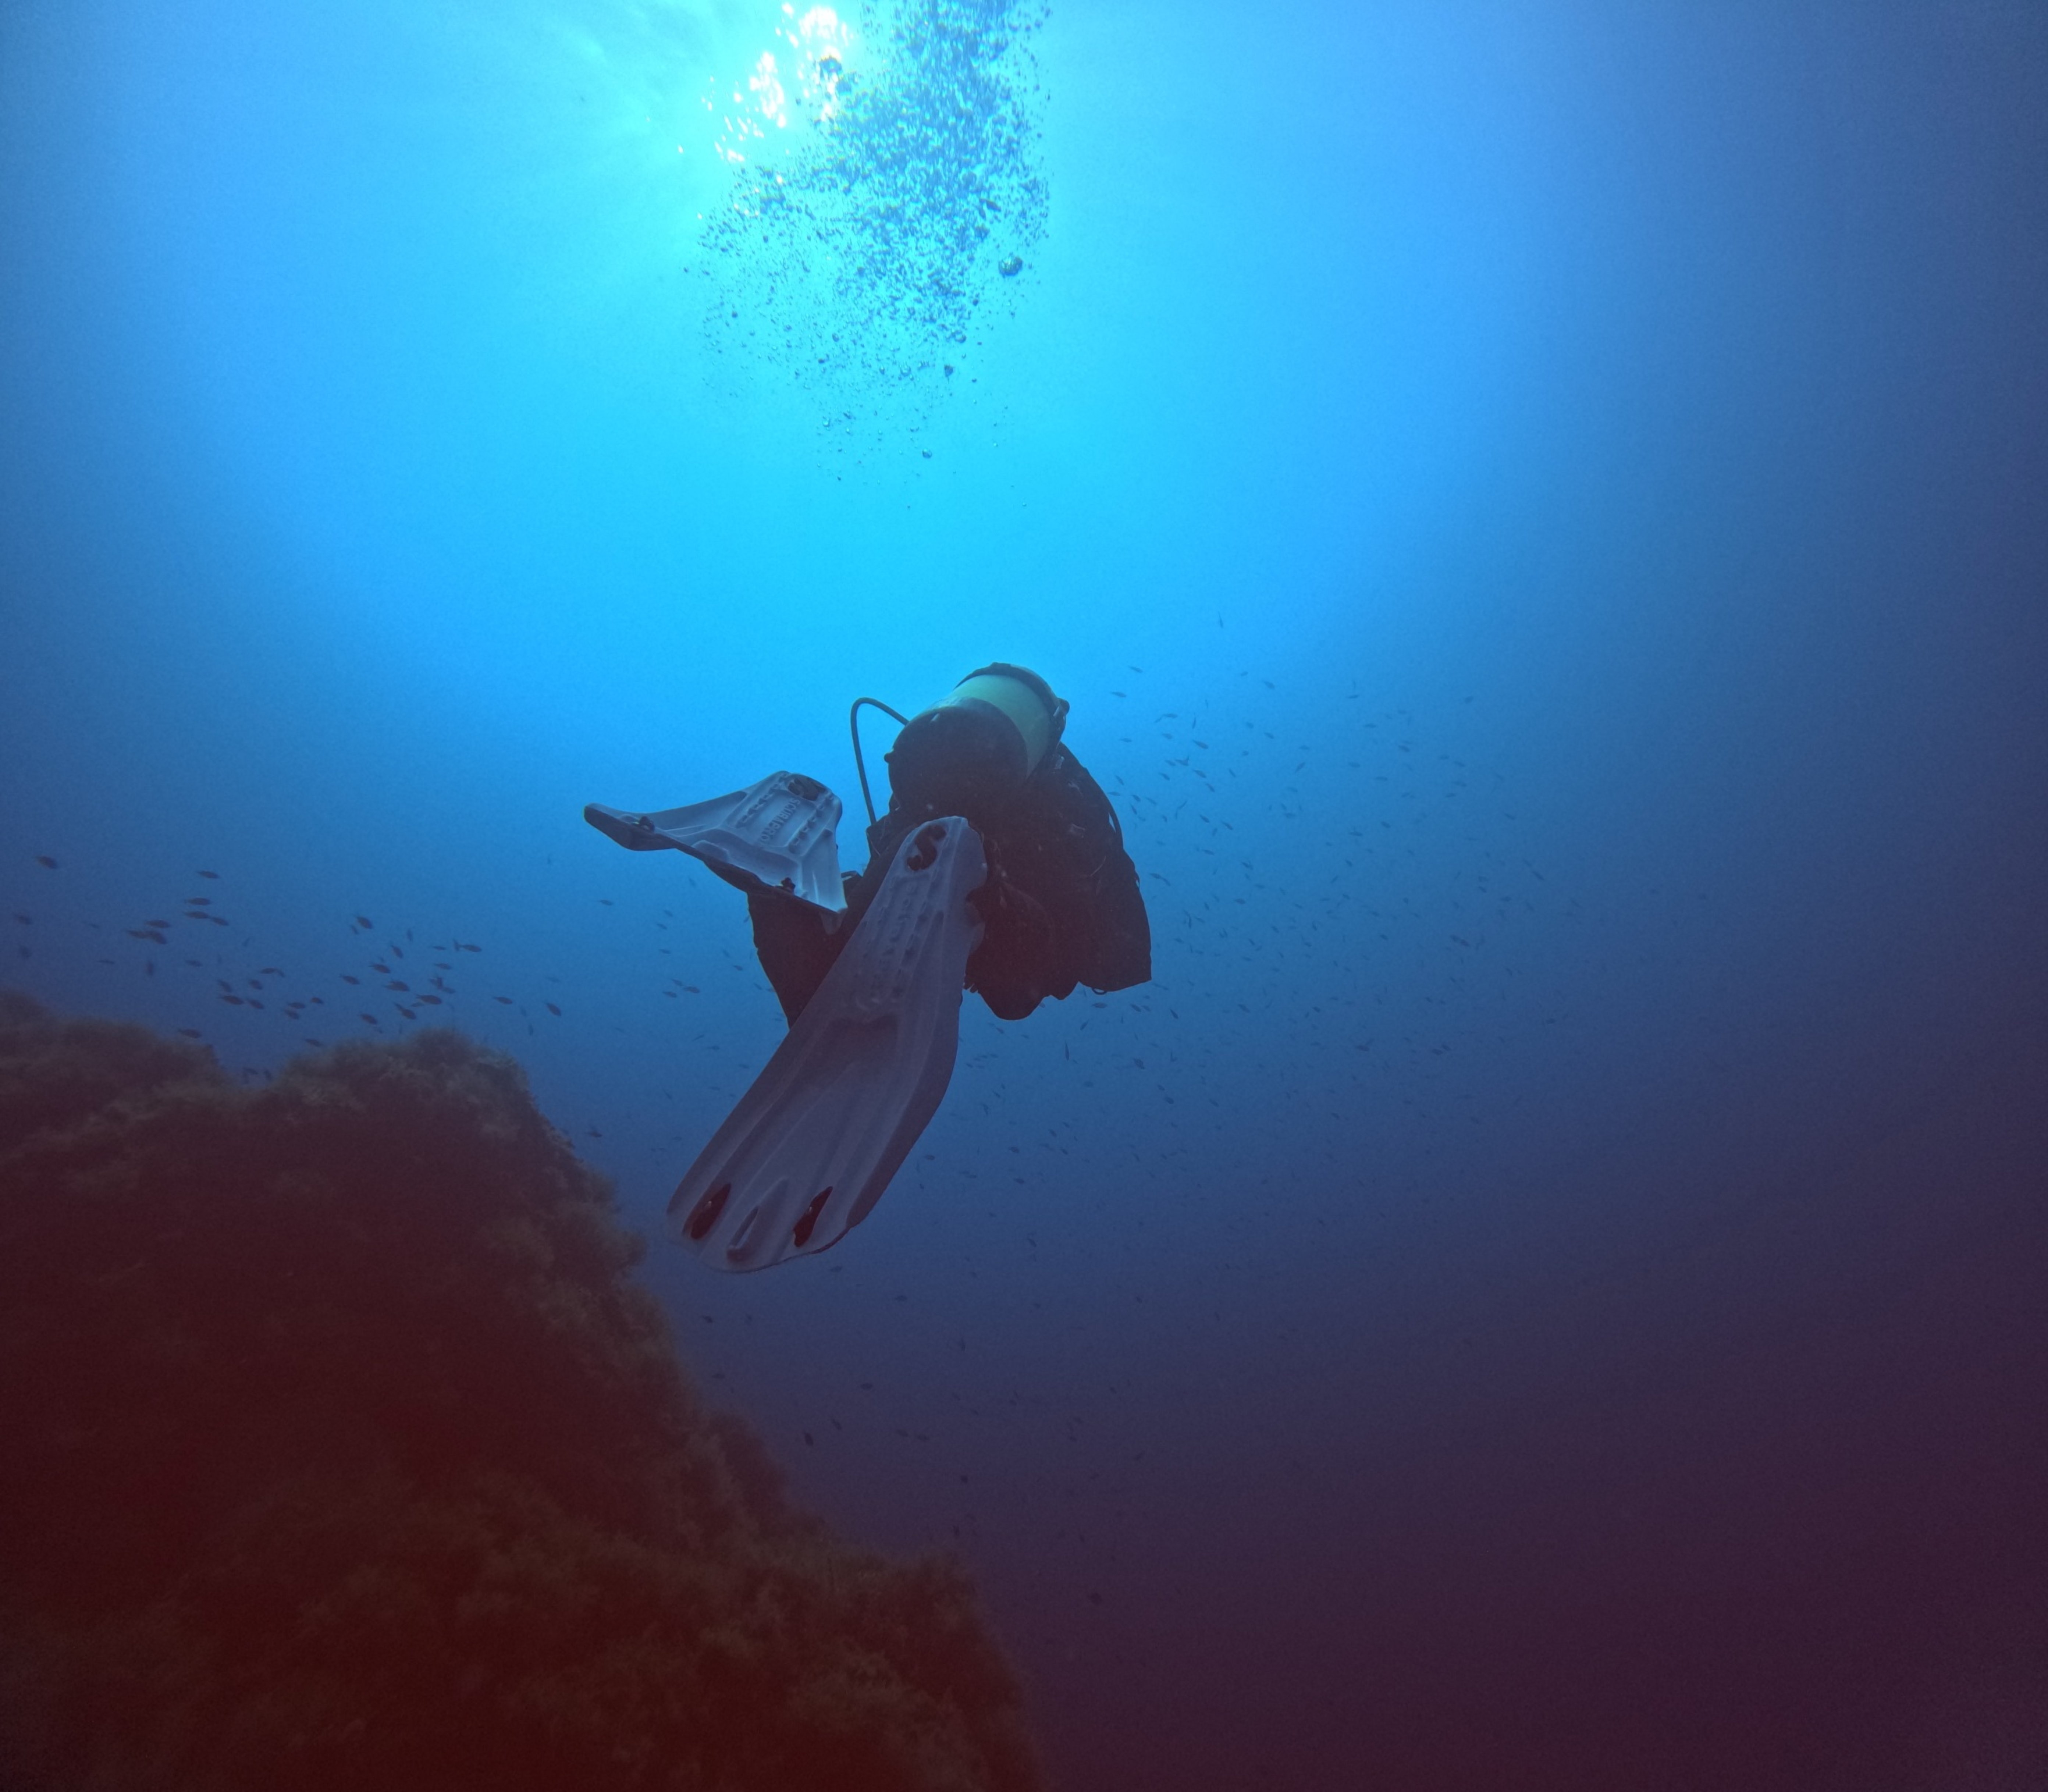
\includegraphics[width=5cm]{res/img}
			\label{label_sous_figure_3}
		}\\
		\subfloat[sous-légende 4]{
			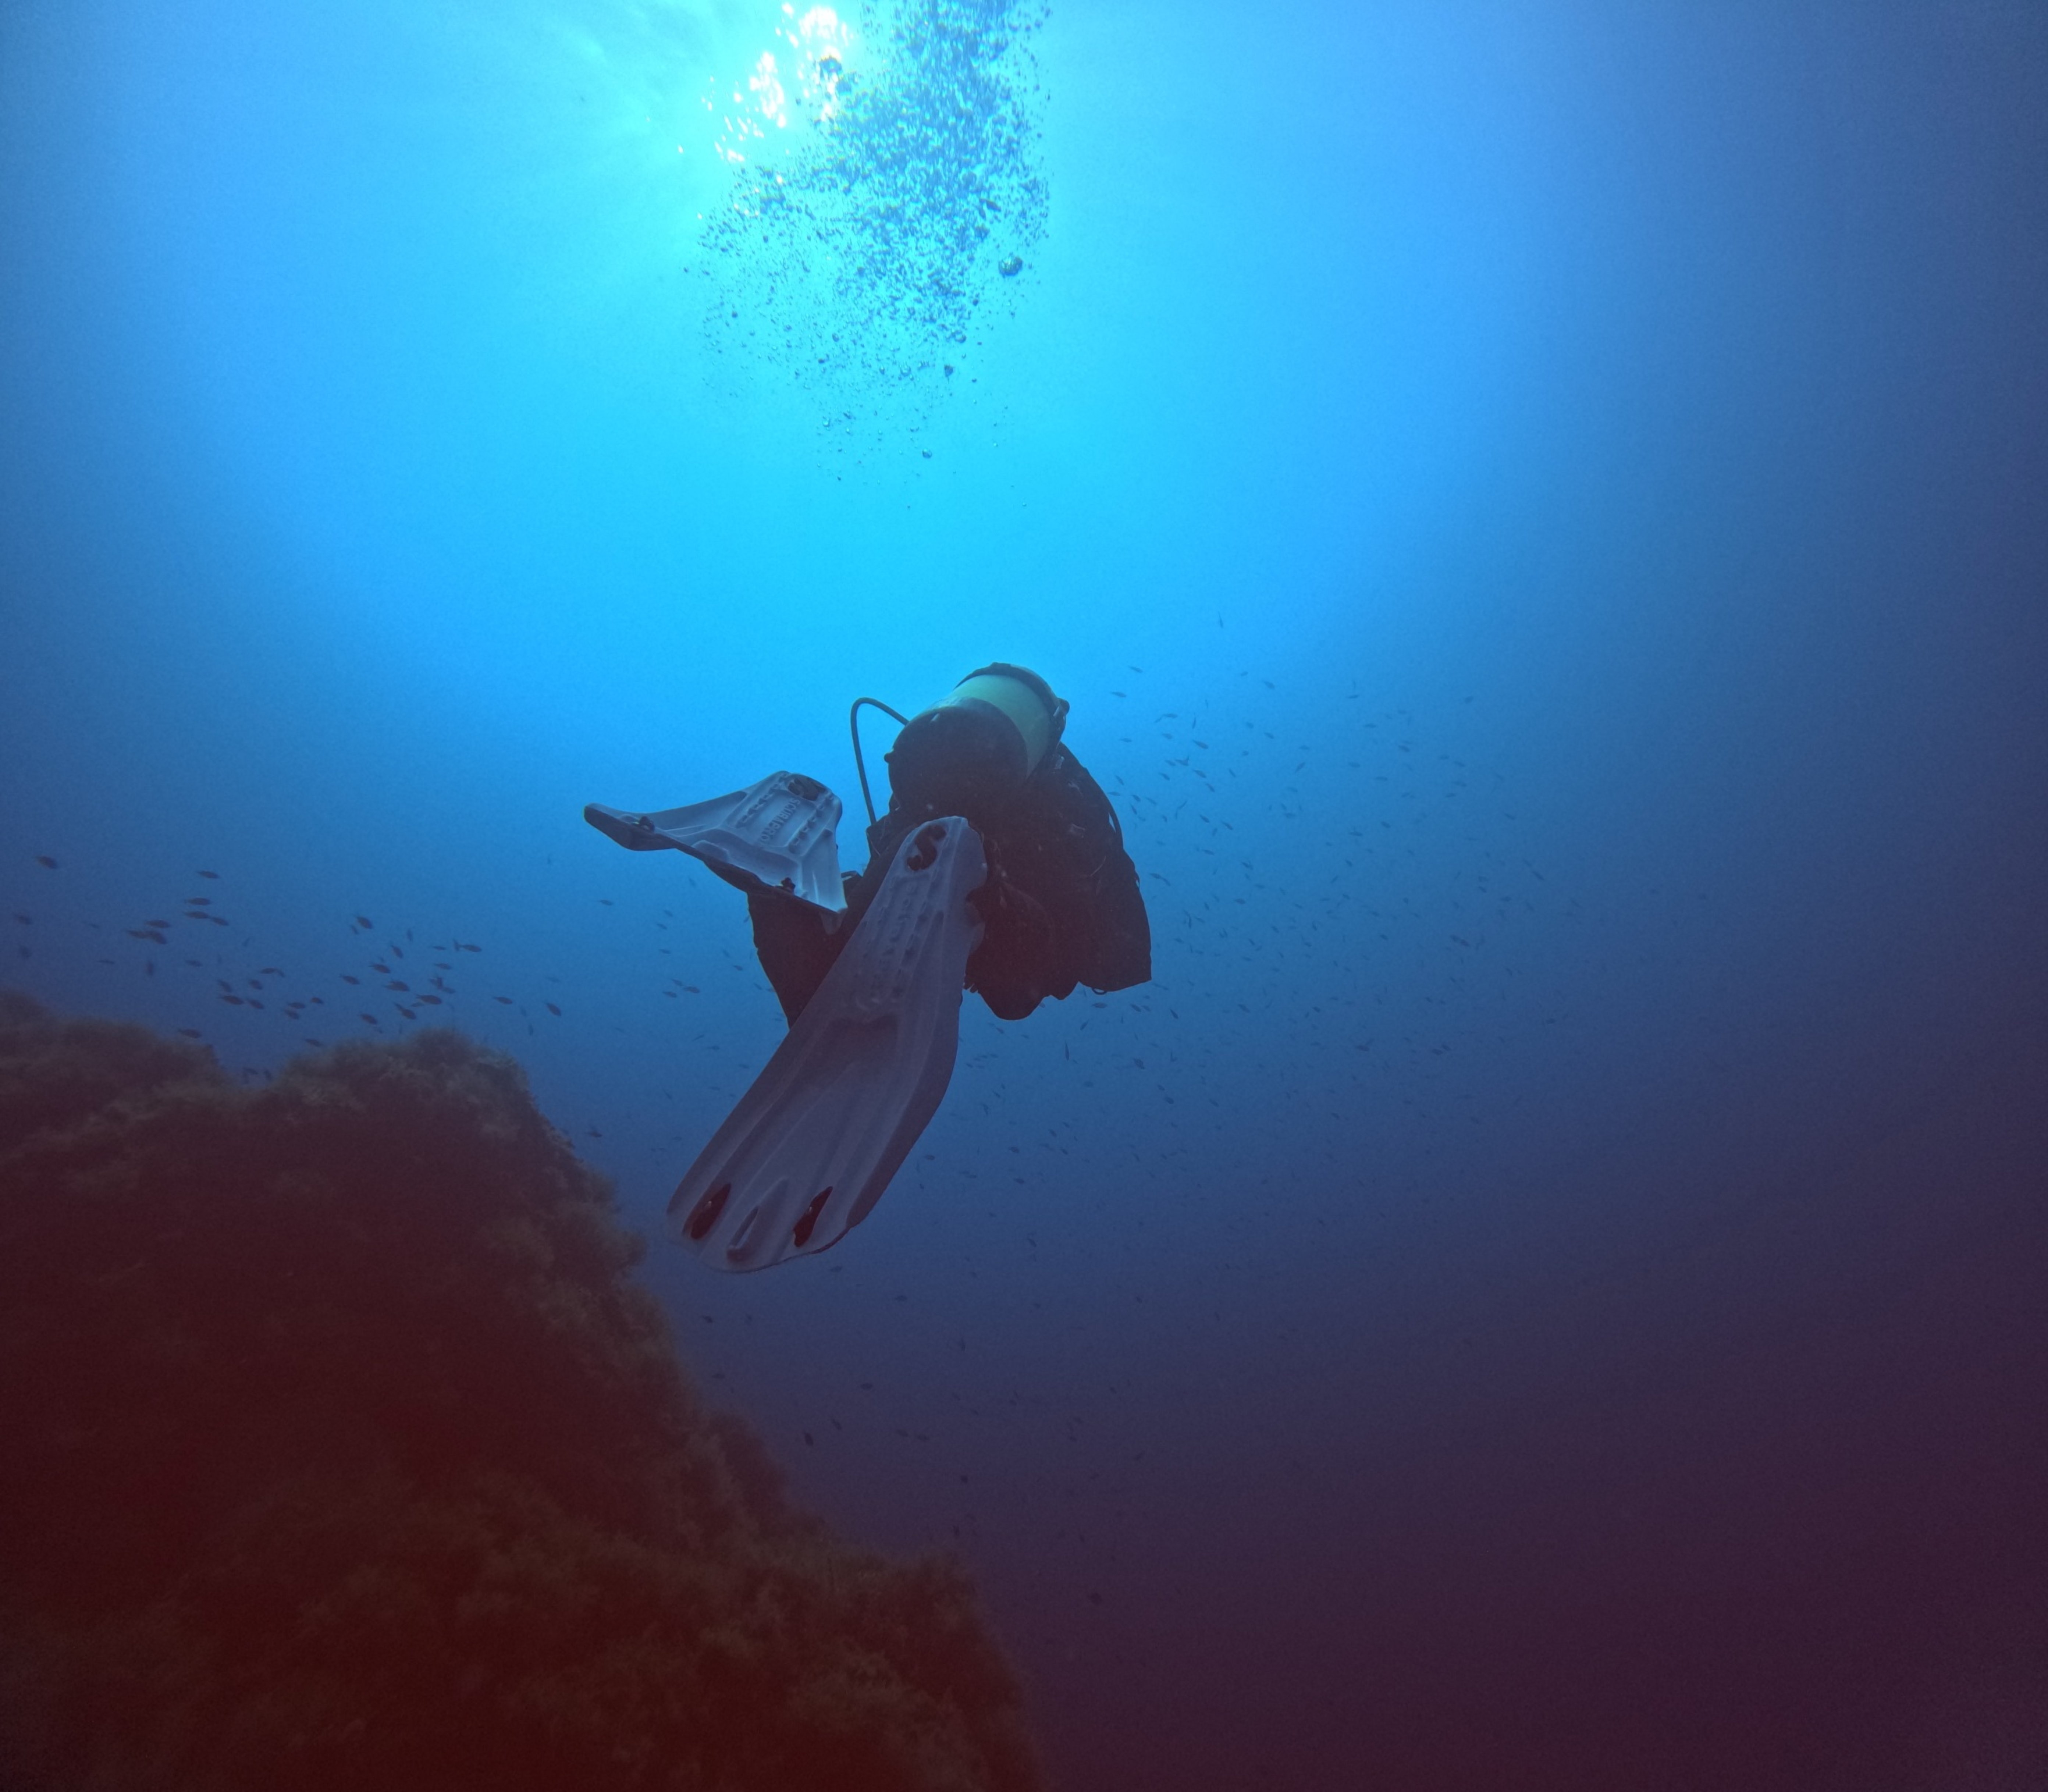
\includegraphics[height=70mm]{res/img}
			\label{label_sous_figure_4}
		}\\
		\caption{Légende globale des 4 figures}\label{label_general}
	\end{figure}

%
% pdfpages : insertion de pages de pdf : https://la-bibliotex.fr/2019/01/31/package-latex-decouverte-1/
%
% \includepdf[pages=0,lastpage=0]{qr}

\chapter{Code}
	En Python \faPython, on utilise \mintinline{python}|for| pour les boucles bornées et \mintinline{python}|while| pour les boucles non bornées.

	\begin{cbox}{un bout de code C}
		\begin{minted}[autogobble,breaklines,linenos,numbersep=10mm]{c}
			#include <stdio.h>

			int main ( int argc, char *argv[] )
			{
				printf ( "hello world\n" );
				return 0;
			}
		\end{minted}
	\end{cbox}

	\begin{cbox}{un bout de code python}
		\begin{minted}[autogobble,breaklines,linenos,numbersep=10mm]{python}
			# Une première boucle
			for i in range(0,5):
				print(i)
		\end{minted}
	\end{cbox}

	\begin{cbox}{un bout de code JS}
		\begin{minted}[autogobble]{js}
			Array.prototype.distinct = function () { return Array.from ( new Set ( this ) ); };
		\end{minted}
	\end{cbox}

%
% https://fr.overleaf.com/learn/latex/LaTeX_Graphics_using_TikZ%3A_A_Tutorial_for_Beginners_(Part_3)%E2%80%94Creating_Flowcharts
%
\chapter{Algorithme}
	\begin{tikzpicture}[node distance=2cm]
		\node (start) [startstop] {Start};
		\node (in1) [io, below of=start] {Input};
		\node (pro1) [process, below of=in1] {Process 1};
		\node (dec1) [decision, below of=pro1] {Decision 1};
		\node (pro2b) [process, right of=dec1, xshift=2cm] {Process 2b};
		\node (pro2a) [process, below of=dec1, yshift=-0.5cm] {Process 2a, avec du text};
		\node (out1) [io, below of=pro2a] {Output};
		\node (stop) [startstop, below of=out1] {Stop};

		\draw [arrow] (start) -- (in1);
		\draw [arrow] (in1) -- (pro1);
		\draw [arrow] (pro1) -- (dec1);
		\draw [arrow] (dec1) -- (pro2a);
		\draw [arrow] (dec1) -- (pro2b);
		\draw [arrow] (dec1) -- node[anchor=east] {yes} (pro2a);
		\draw [arrow] (dec1) -- node[anchor=south] {no} (pro2b);
		\draw [arrow] (pro2a) -- (out1);
		\draw [arrow] (out1) -- (stop);

		\draw [arrow] (pro2b) |- (pro1);
	\end{tikzpicture}

\chapter{Tableaux}
	\begin{tabular}{|l|p{0.5\linewidth}|c|r |}
		\hline
		left & size & center & right \\
		\hline
		a & a & a & a \\
		a & a & a & a \\
		a & a & a & a \\
		a & a & a & a \\
		\hline
	\end{tabular}

\chapter{Listes} \label{ref_A}
	\begin{itemize}
		\item a
		\item a
		\item a
		\item a
		\item a
	\end{itemize}

\chapter{Références}
	Référence à un chaptre ou section \ref{ref_A} page : \pageref{ref_A}

	Référence à une figure \ref{label_general} ou à une autre \ref{label_sous_figure_3}.

	Référence à un livre / article de bibliographie \cite{id-12}

\chapter{Mail}
	\begin{mail}
		{Objet}
		{sender@domain.com}
		{receveur@domain.fr}
		{date}
		contenu du mail
	\end{mail}

\chapter{Extraits}
	\begin{extraitR}{auteur}
		text issue à ecrire
	\end{extraitR}
	\begin{extraitL}{auteur}
		text issue à ecrire
	\end{extraitL}



%
% https://fr.overleaf.com/learn/latex/LaTeX_Graphics_using_TikZ%3A_A_Tutorial_for_Beginners_(Part_4)%E2%80%94Circuit_Diagrams_Using_Circuitikz
% https://nboulaire.developpez.com/tutoriels/latex/circuitikz_base/
%
\chapter{Circuit electronique}
	\section{compasant}
		\begin{tikzpicture}
			\draw
			[gray] (-2,-2) grid (6,10)
			;
			% (horizontal,vertical)
			\draw (0,0) node[antenna] {};
			\draw (4,0) node[pmos] {};
			\draw (0,4) node[op amp] {};
			\draw (4,4) node[american or port] {};
			\draw (0,8) node[transformer] {};
			\draw (4,8) node[spdt] {};
		\end{tikzpicture}

		\begin{circuitikz}
			\draw
			(0,0) to[R, o-o] (2,0)
			(4,0) to[vR, o-o] (6,0)
			(0,2) to[transmission line, o-o] (2,2)
			(4,2) to[closing switch, o-o] (6,2)
			(0,4) to[european current source, o-o] (2,4)
			(4,4) to[european voltage source, o-o] (6,4)
			(0,6) to[empty diode, o-o] (2,6)
			(4,6) to[full led, o-o] (6,6)
			(0,8) to[generic, o-o] (2,8)
			(4,8) to[sinusoidal voltage source, o-o] (6,8)
			;
		\end{circuitikz}

	\section{simple shema}
		\begin{circuitikz}[scale=0.5]
			\draw
			(0,0)
				to[battery]
			(0,2)
				to [vsource, l=\SI{6}{V}, v_=$U_G$]
			(0,4)
				to[ammeter, i_=2<\milli\ampere>]
			(4,4)
				to[C]
			(4,0)
				--
			(3.5,0)
				to[lamp, *-*]
			(0.5,0)
				--
			(0,0)
			;
			\draw
			(0.5,0)
				--
			(0.5,-2)
				to[voltmeter, v_=2<\kilo\volt>, color=red]
			(3.5,-2)
				--
			(3.5,0)
			;
			\draw
			(0.5,-2)
				--
			(0.5,-4)
				to[ohmmeter, color=green, o-*]
			(3.5,-4)
				--
			(3.5,-2)
			;
		\end{circuitikz}

	\section{composant plus complexes}
		\begin{circuitikz}
			\draw
			(0, 0)
				node[op amp] (opamp1) {}
			(4, -2)
				node[op amp] (opamp2) {}
			(opamp1.-)
				to [R]
			(-3, 0.5)

			(opamp1.out)
				-|
			(opamp2.-)

			(opamp1.-)
				|-
			(-1,2)
				to [C]
			(1,2) 
				-|
			(opamp1.out) node[right] {$A$}
			;
			% façon de rajouter les point de connexions sur les T
	            \draw[fill=black] (opamp1.-) circle (1.5pt);
	            \draw[fill=black] (opamp1.out) circle (1.5pt);
		\end{circuitikz}

	\section{circuit complexe complet}
		\begin{circuitikz}
			\tikzset{every pin/.append style={pin distance=11mm,
			                                  pin edge={<-,shorten <=2pt,semithick,cyan},
			                                  align=center, text=cyan}}
			\ctikzset{bipoles/length=1cm}
			\draw   (0,0)   node[below] {$+$}
			                to [short,i=\textcolor{cyan}{$i_1{=}\frac{v_I}{R_1}$},o-]    ++ (1,0)
			                to [R=$R_1$,-*] ++ (2.0,0)
			                coordinate[pin={[xshift=1em]240:{$v_I=0$}\\ (Virtual ground)}] (aux1)
			                to [short,i=\textcolor{cyan}{$i_1{=}0$}]    ++ (1,0)
			                node [op amp, anchor=-] (amp) {}
			        (aux1)  -- ++ (0,2)
			                to [short,i=\textcolor{cyan}{$i_2{=}i_1=\frac{v_I}{R_1}$}]    ++ (1,0)
			                to [R=$R_2$]    ++ (2,0)
			                |- (amp.out)
			                to [short,-o]   ++ (2,0)
			                node[below] {$+$}
			                to [open,l=\textcolor{cyan}{$v_o{=}0-\frac{v_1}{R_1}$}] ++ (0,-2)
			                node[ground,label=$-$] (aux2) {}
			        (amp.+) -| (aux1 |- aux2)
			                node[ground] {}
			        (0,0)   to [open,l_=\textcolor{cyan}{$v_I$}] (0,0 |- aux2)
			                node[ground,label=$-$] (aux2) {}
			        ;
		\end{circuitikz}